\documentclass[14pt,a4paper]{extreport}

\usepackage[left=30mm, top=20mm, right=10mm, bottom=20mm]{geometry}
\usepackage{cmap}		
\usepackage[utf8]{inputenc}
\usepackage[english, russian]{babel}
\usepackage{framed}
\usepackage{amsmath}
\usepackage{graphicx}
\usepackage{wrapfig}
\usepackage{listings}
\usepackage{color}
\usepackage{indentfirst}
\usepackage{textcomp}
\usepackage{titlesec}
\usepackage{alltt}

\usepackage{cite}
\usepackage{url}
%%%%%%%%%%%%%%%%%%%%%%%%%%%%%%%%%%%%%%%%%%%%%%%%%%%%%%%%%%%%%%%%%%%%%%%%

\titleformat{\chapter}[display]
    {\filcenter\large\bfseries}
    {\MakeUppercase{\chaptertitlename} \thechapter}
    {8pt}
    {\bfseries}{}
\titleformat{\section}
    {\normalsize\bfseries}
    {\thesection}
    {1em}{}
\titleformat{\subsection}
    {\normalsize\bfseries}
    {\thesubsection}
    {1em}{}

%% Настройка вертикальных и горизонтальных отступов
\titlespacing*{\chapter}{0pt}{-30pt}{8pt}
\titlespacing*{\section}{\parindent}{*4}{*4}
\titlespacing*{\subsection}{\parindent}{*4}{*4}

%% Отступ от левого края
\oddsidemargin=0pt 

\lstdefinestyle{customc}{belowcaptionskip=1\baselineskip,breaklines=true,frame=L,xleftmargin=\parindent,  language=C, showstringspaces=false, basicstyle=\footnotesize\ttfamily,keywordstyle=\bfseries\color{green!40!black},  commentstyle=\itshape\color{purple!40!black}, identifierstyle=\color{blue}, stringstyle=\color{orange},numbers=left,numbersep=12pt, numberstyle=\small\color{mygray},}
\lstset{escapechar=@,style=customc}

\newcommand{\HRule}{\rule{\linewidth}{0.5mm}}

\begin{document}

%% Титульный
%%%%%%%%%%%%%%%%%%%%%%%%%%%%%%%%%%%%%%%%%%%%%%%%%%%%%%%%%%%%%%%%%%%%%%%%
\begin{titlepage}
\begin{center}


{\normalsize 
Федеральное государственное автономное образовательное учреждение высшего образования 
\\Санкт-Петербургский национальный исследовательский университет 
\\информационных технологий, механики и оптики}

\vspace{1.5cm}

\vspace{0.5cm}
\large Факультет систем управления и робототехники
% Upper part of the page. The '~' is needed because \\
% only works if a paragraph has started.
%\includegraphics[width=0.18\textwidth]{img/logo.png}~\\[1cm]
\vspace{2cm}

\large Курсовой проект
\\ Вариант №2

по дисциплине <<Программирование систем управления>>

{ \large \bfseries <<Моделирование системы управления>>\\[0.4cm] }

% Author and supervisor
\noindent

\begin{flushright} \normalsize
\emph{Выполнили:}\\
Студент группы R41332\\
Волков \textsc{А.~А.}\\
% Щербаков \textsc{П.~В.}\\

\emph{Проверил:} \\
Томашевич \textsc{С.~И.}
\end{flushright}

\vfill

% Bottom of the page
{\normalsize Санк-Петербург, 2019 г.}

\end{center}
\end{titlepage}

%%%%%%%%%%%%%%%%%%%%%%%%%%%%%%%%%%%%%%%%%%%%%%%%%%%%%%%%%%%%%%%%%%%%%%%%

%% Оглавление
%%%%%%%%%%%%%%%%%%%%%%%%%%%%%%%%%%%%%%%%%%%%%%%%%%%%%%%%%%%%%%%%%%%%%%%%
\newpage
\tableofcontents
%%%%%%%%%%%%%%%%%%%%%%%%%%%%%%%%%%%%%%%%%%%%%%%%%%%%%%%%%%%%%%%%%%%%%%%%

%% Задание
%%%%%%%%%%%%%%%%%%%%%%%%%%%%%%%%%%%%%%%%%%%%%%%%%%%%%%%%%%%%%%%%%%%%%%%%
\chapter*{Задание}
\addcontentsline{toc}{chapter}{Задание}

\begin{enumerate}
\item
Реализовать класс интегратора в .cpp и .h файлах.
    
\item 
Привести задающее воздействие в виде модели с использованием интегратором.
    
\item 
Дисретизировать полученные модели задающего воздействия 
и объекта управления с шагами дискретизации 5, 50, 100 Гц.

\item
Программно реализовать отдельными классами четыре случая объектов 
(непрерывный и три дискретных). Для дискретных случаев сделать 
реализацию с использованием разностных уравнений.
\begin{equation} 
    x_{k+1} = A \cdot x_k
\end{equation}
То есть интегратор заменяется на элемент памяти.

\item 
Добавить реализованные классы в предоставленную программу для \\ QtCreator.

\item
Поочередно провести сравнение поведений реализованных непрерывв-
ных моделей с дискретными моделями с соответствующими шагами
дискретизации. Шаг дискретизации меняется в предоставленной про-
грамме. В результате должно получиться три пары сравнений.

\item 
В предоставленной программе QtCreator настроить последовательный
порт (qSerialPort) на скорость 115200 бод, формат 8N1.

\item 
Закодировать с помощью метода COBS значения, полученные с выхода
объекта в следующем формате:
{[0x0A 0xXX 0xXX 0xXX 0xXX 0xCR]}, где 0xXX – байты полученного 
числа с плавающей точкой (float) в
обратном порядке, а 0xCR – проверочная сумма, равная сумме всех
остальных байт сообщения, вычтенной из 0xFF.

\end{enumerate}
%%%%%%%%%%%%%%%%%%%%%%%%%%%%%%%%%%%%%%%%%%%%%%%%%%%%%%%%%%%%%%%%%%%%%%%%

%% Исходные данные
%%%%%%%%%%%%%%%%%%%%%%%%%%%%%%%%%%%%%%%%%%%%%%%%%%%%%%%%%%%%%%%%%%%%%%%%
\newpage
\chapter*{Исходные данные}
\addcontentsline{toc}{chapter}{Исходные данные}

\begin{equation}
    u(t) = 3 \cdot  cos(0.1 \cdot t + 1)
\end{equation}

\begin{equation}
    A = 
    \begin{bmatrix} 
        0 & 1 & 0 \\ 
        0 & 0 & 1 \\
        -1.5 & -5 & -2
    \end{bmatrix}
\end{equation}

\begin{equation}
    B = 
    \begin{bmatrix} 
        0 \\ 
        0 \\
        1
    \end{bmatrix}
\end{equation}

\begin{equation}
    C = 
    \begin{bmatrix} 
        0.5 & 0 & 0
    \end{bmatrix}
\end{equation}

\begin{equation}
\dot x = A \cdot x + B \cdot u(t)
\end{equation}

\begin{equation}
y = C \cdot x
\end{equation}
%%%%%%%%%%%%%%%%%%%%%%%%%%%%%%%%%%%%%%%%%%%%%%%%%%%%%%%%%%%%%%%%%%%%%%%%

%% Ход работы
%%%%%%%%%%%%%%%%%%%%%%%%%%%%%%%%%%%%%%%%%%%%%%%%%%%%%%%%%%%%%%%%%%%%%%%%
\chapter*{Ход работы}
\addcontentsline{toc}{chapter}{Ход работы}
Исходный код программы представлен в приложении А. 

Программно реализовать отдельными классами четыре случая объектов 
(непрерывный и три дискретных). Для дискретных случаев сделать 
реализацию с использованием разностных уравнений.

Переходной процесс непрерывной системы 
представлен на рис.\ref{fig:contin}.
\begin{figure}[h]
    \centering
    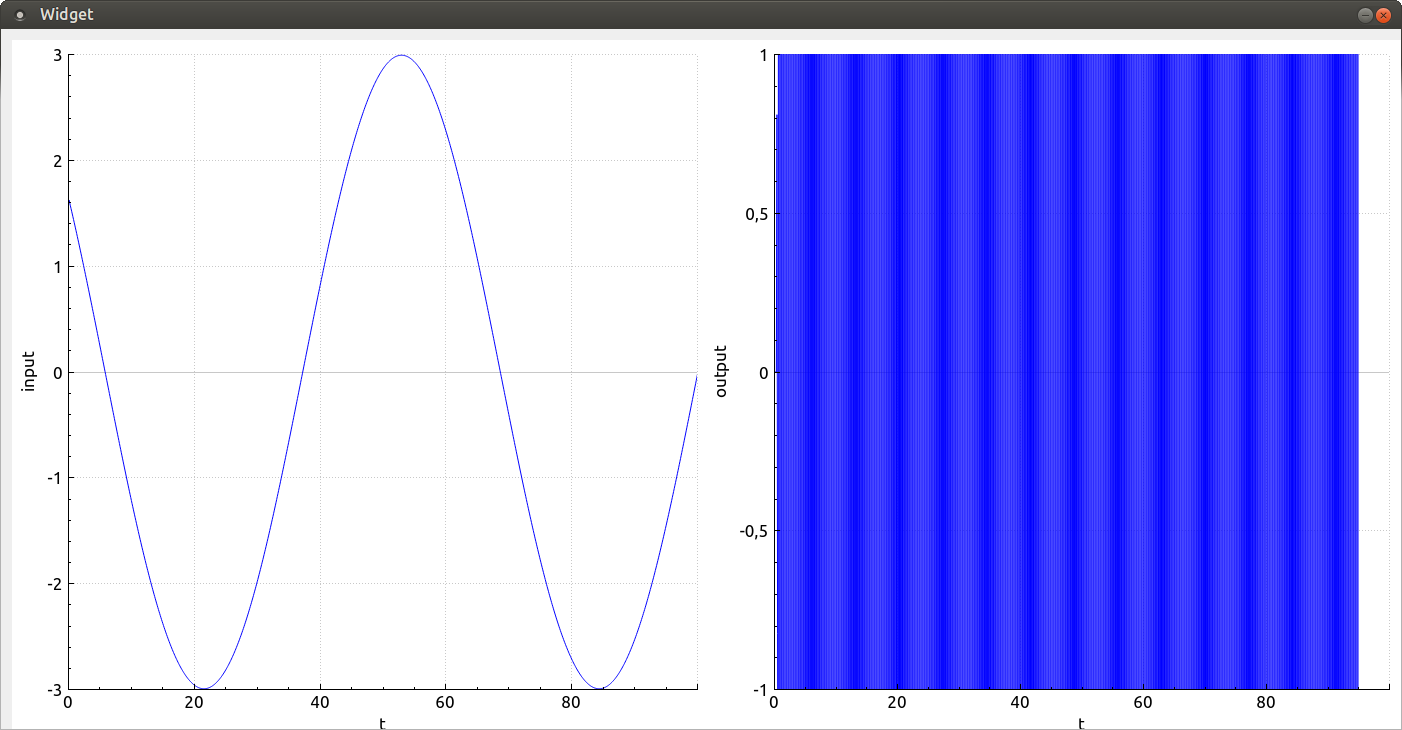
\includegraphics[width=160mm]{img/cont.png}
    \caption{Переходной процесс непрерывной системы}
    \label{fig:contin}
\end{figure}

Переходной процесс дискретной системы с шагом дискретизации 
5 Гц представлен на рис.\ref{fig:discrete5}.

\begin{figure}[h]
    \centering
    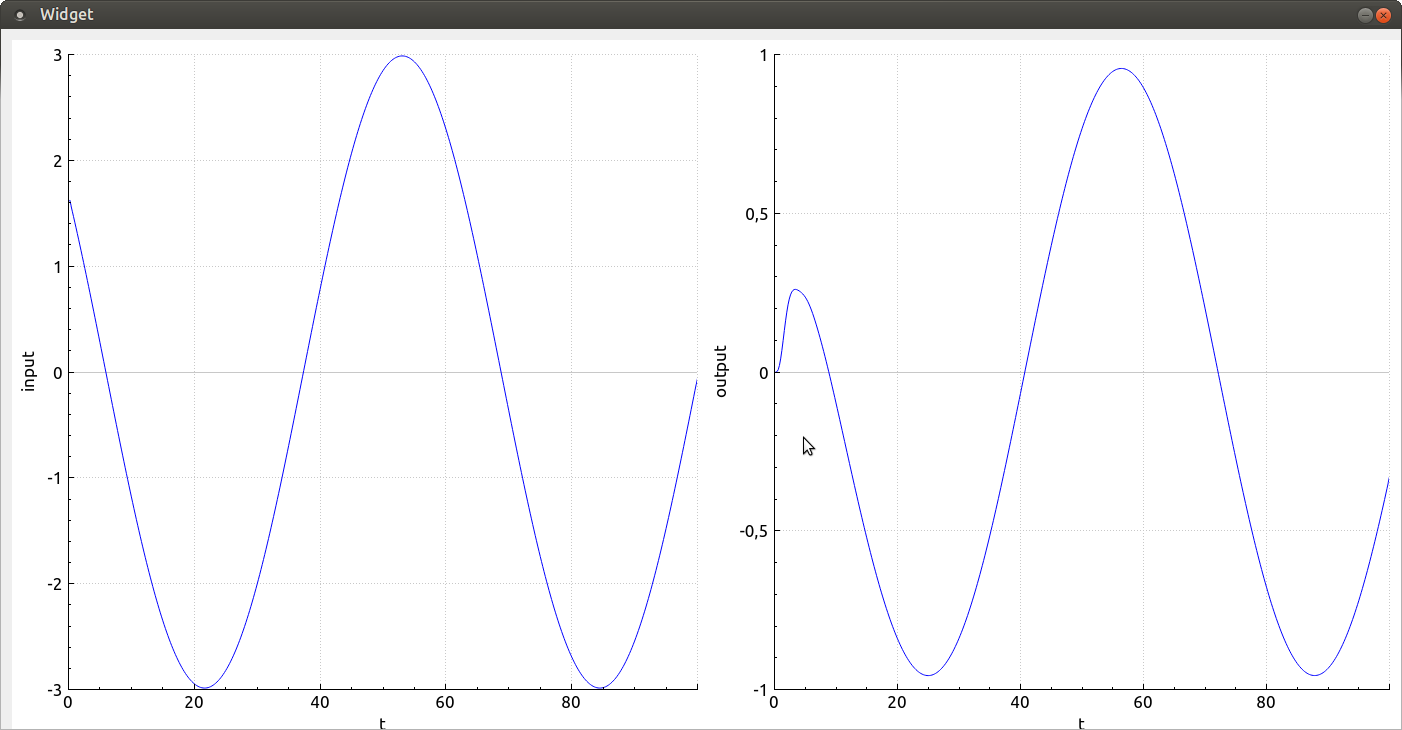
\includegraphics[width=160mm]{img/5hz.png}
    \caption{Переходной процесс дискретной системы 
    с шагом дискретизации 5 Гц}
    \label{fig:discrete5}
\end{figure}

Переходной процесс дискретной системы с шагом дискретизации 
50 Гц представлен на рис.\ref{fig:discrete50}.

\begin{figure}[h]
    \centering
    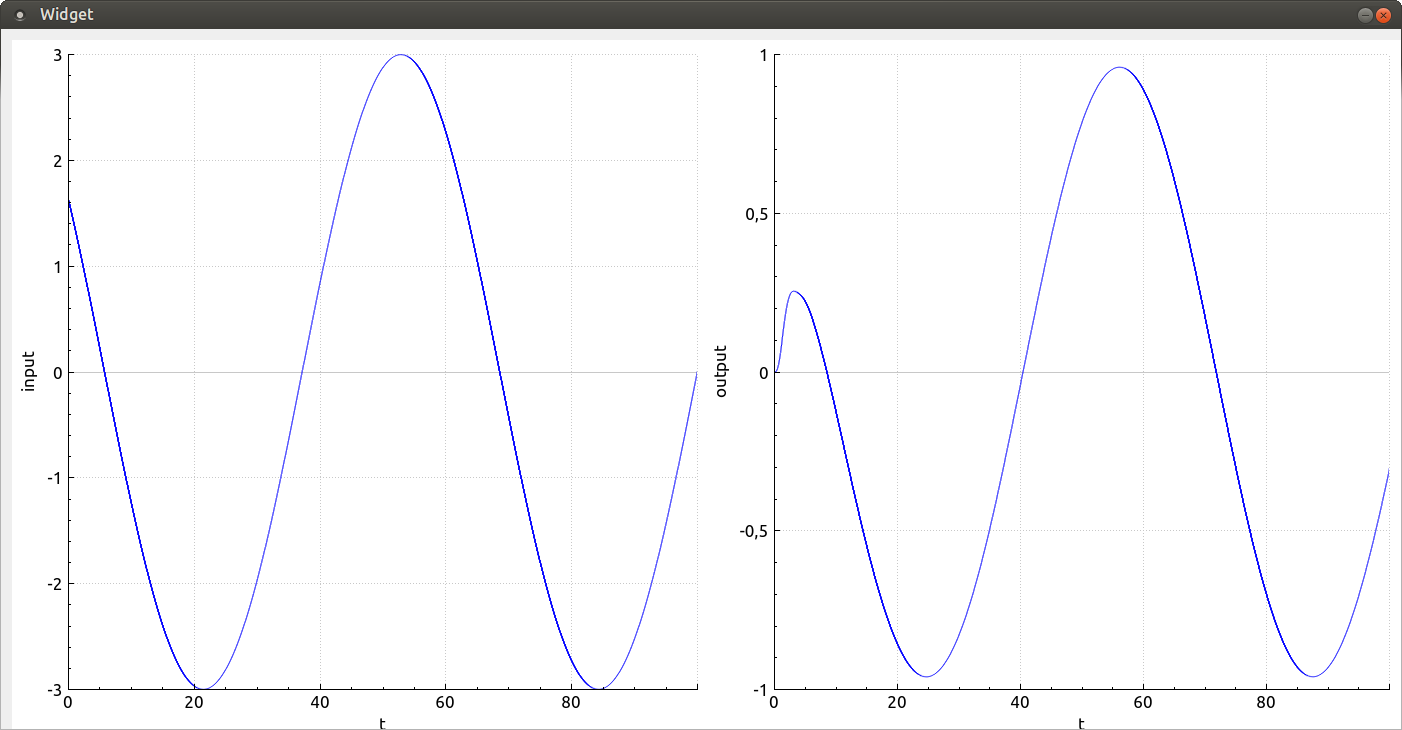
\includegraphics[width=160mm]{img/50hz.png}
    \caption{Переходной процесс дискретной системы 
    с шагом дискретизации 50 Гц}
    \label{fig:discrete50}
\end{figure}

Переходной процесс дискретной системы с шагом дискретизации 
100 Гц представлен на рис.\ref{fig:discrete100}.

\begin{figure}[h]
    \centering
    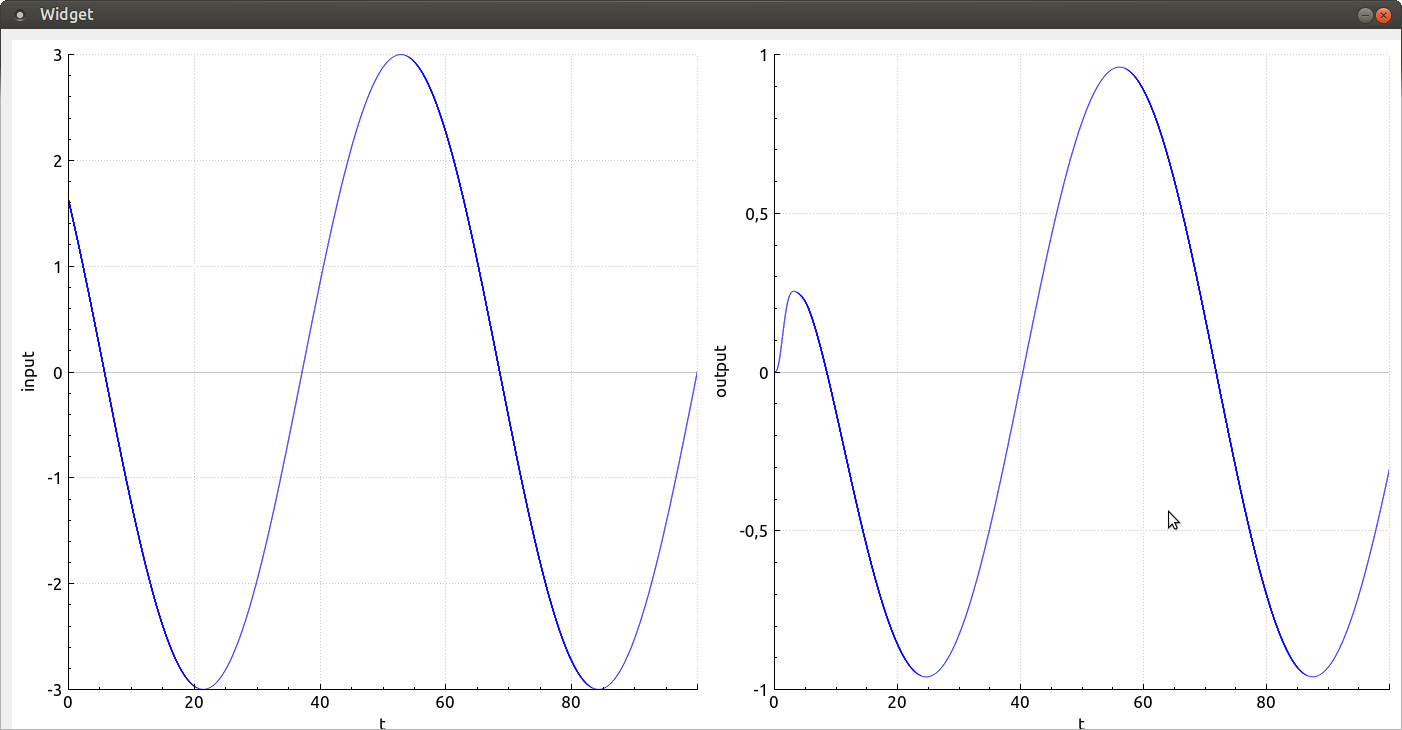
\includegraphics[width=160mm]{img/100hz.png}
    \caption{Переходной процесс дискретной системы 
    с шагом дискретизации 100 Гц}
    \label{fig:discrete100}
\end{figure}

%%%%%%%%%%%%%%%%%%%%%%%%%%%%%%%%%%%%%%%%%%%%%%%%%%%%%%%%%%%%%%%%%%%%%%%%

%% Приложение А. Исходный код программы
%%%%%%%%%%%%%%%%%%%%%%%%%%%%%%%%%%%%%%%%%%%%%%%%%%%%%%%%%%%%%%%%%%%%%%%%
\newpage
\chapter*{Приложение А. Исходный код программы}
\addcontentsline{toc}{chapter}{Приложение А. Исходный код программы}

%%%%%%%%%%%%%%%%%%%%%%%%%%%%%%%%%%%%%%%%%%%%%%%%%%%%%%%%%%%%%%%%%%%%%%%%
\textbf{Файл model.cpp}
\begin{alltt}
\begin{verbatim}
#include "model.h"

Model::Model() {
    ///
    ///////////////////////////////////////////////////////////
    double _In[] = {1, 0, 0, 0, 1, 0, 0, 0, 1};
    Matrix In(3, 3, _In);

    double _A[] = {0, 1, 0, 0, 0, 1, -1.5, -5, -2};
    Matrix A = Matrix(3, 3, _A);

    this->Ad = A.matExp(TIME_STEP);

    double _B[] = {0, 0, 1};
    Matrix B = Matrix(3, 1, _B);
    this->Bd = A.inverse()*(Ad - In)*B;

    double _C[] = {0.5, 0, 0};
    Matrix C = Matrix(1, 3, _C);
    this->Cd = C;

    double _x[] = {0, 0, 0};
    this->x = Matrix(3, 1, _x);

    this->y = Matrix(1, 1);

    /// cos(1)*amplitude
    /// -sin(1rad)*omega*amplitude
    double _u_state[] = {0.54*3, 0.84147*-0.3};
    this->u_state = Matrix(2, 1, _u_state);
    ///////////////////////////////////////////////////////////
    
    ///
    ///////////////////////////////////////////////////////////
    this->serial_port.setPortName(this->SERIAL_PORT_NAME);
    this->serial_port.setBaudRate(this->SERIAL_PORT_BAUD_RATE);

    // if (!serial_port.open(QIODevice::WriteOnly)) {
    //     std::cout << "Can not open port" << std::endl;
    // }
    ///////////////////////////////////////////////////////////
}

Model::~Model() {
    serial_port.close();
}

void Model::send(const double& value) {
    std::stringstream os;
    os << value;
    QByteArray write_data(os.str().c_str());
    qint64 bytes_written = serial_port.write(write_data);

    if (bytes_written == -1) {
        std::cout << "Failed to write the data" << std::endl;
    } else if (bytes_written != write_data.size()) {
        std::cout << "Failed to write all the data" << std::endl;
    } else if (!serial_port.waitForBytesWritten(5000)) {
        std::cout << "Operation timed out or an error" << std::endl;  
    }
}

double Model::update(const double& input) {
    x_prev = x;
    x = Ad*x + Bd*input;
    y = Cd*x_prev;

    double output = this->y.getM();

    return output;
}

double Model::control() {
    /// Constants
    ///////////////////////////////////////////////////////////
    const double T = this->TIME_STEP;

    const double _In[] = {1, 0, 0, 1};
    const Matrix In(2, 2, _In);

    const double _u_A[] = {0, -1, OMEGA*OMEGA, 0};
    const Matrix u_A = Matrix(2, 2, _u_A);
    ///////////////////////////////////////////////////////////

    ///////////////////////////////////////////////////////////
    Matrix mat_exp = Matrix(2, 1);
    Matrix u = Matrix(2, 1);
    
    double signal = _u_state.getState();

    this->_du_state.update(feedback, T);
    this->_u_state.update(_du_state.getState(), T);
    
    feedback = -OMEGA*OMEGA*_u_state.getState();
    ///////////////////////////////////////////////////////////

    return signal;
}
    
\end{verbatim}
\end{alltt}
%%%%%%%%%%%%%%%%%%%%%%%%%%%%%%%%%%%%%%%%%%%%%%%%%%%%%%%%%%%%%%%%%%%%%%%%

%%%%%%%%%%%%%%%%%%%%%%%%%%%%%%%%%%%%%%%%%%%%%%%%%%%%%%%%%%%%%%%%%%%%%%%%
\textbf{Файл model.h}
\begin{alltt}
\begin{verbatim}
#ifndef MODEL_H
#define MODEL_H

#include <iostream>
#include <inttypes.h>
#include <QSerialPort>
#include <sstream>

#include "matrix.h"
#include "integrator.h"

class Model
{
/// Attributes
///////////////////////////////////////////////////////////
private:
    const double OMEGA = 0.1;
    const QString SERIAL_PORT_NAME = "/dev/pts/11";
    const int SERIAL_PORT_BAUD_RATE = QSerialPort::Baud115200;

    Matrix Ad = Matrix(3, 3);
    Matrix Bd = Matrix(3, 1);
    Matrix Cd = Matrix(1, 3);
    Matrix x = Matrix(3, 1);
    Matrix y = Matrix(1, 1);
    Matrix x_prev = Matrix(3, 1);
    Matrix u_state = Matrix(2, 1);

    Integrator _du_state = Integrator(-3*OMEGA*std::sin(1), 0);
    Integrator _u_state = Integrator(3 * std::cos(1), 0);
    double feedback;

    QSerialPort serial_port;

public:
    const double TIME_STEP = 0.1;
    const double SIMULATION_TIME = 100;
    double time_now = 0;

///////////////////////////////////////////////////////////

/// Methods
///////////////////////////////////////////////////////////
public:
    /// Constructors and destructors
    ///////////////////////////////////////////////////////////
    Model();

    ~Model();
    ///////////////////////////////////////////////////////////

    /// 
    ///////////////////////////////////////////////////////////
    void send(const double& value);

    double update(const double& input);

    double control();
    ///////////////////////////////////////////////////////////
};
#endif // MODEL_H
    
\end{verbatim}
\end{alltt}
%%%%%%%%%%%%%%%%%%%%%%%%%%%%%%%%%%%%%%%%%%%%%%%%%%%%%%%%%%%%%%%%%%%%%%%%

%%%%%%%%%%%%%%%%%%%%%%%%%%%%%%%%%%%%%%%%%%%%%%%%%%%%%%%%%%%%%%%%%%%%%%%%
\textbf{Файл integrator.h}
\begin{alltt}
\begin{verbatim}
class Integrator {

    public:
        Integrator(double init_state, double init_in);
    
        void update(double input, double dt);
    
        double getState_prev();
    
        double getState();
    
    private:
        double state;
        double state_prev;
        double prev_in = 0;
    };
        
\end{verbatim}
\end{alltt}
%%%%%%%%%%%%%%%%%%%%%%%%%%%%%%%%%%%%%%%%%%%%%%%%%%%%%%%%%%%%%%%%%%%%%%%%

%%%%%%%%%%%%%%%%%%%%%%%%%%%%%%%%%%%%%%%%%%%%%%%%%%%%%%%%%%%%%%%%%%%%%%%%
\textbf{Файл integrator.cpp}
\begin{alltt}
\begin{verbatim}
#include "integrator.h"

Integrator::Integrator(double init_state, double init_in): 
    state(init_state),
    prev_in(init_in)
{}

void Integrator::update(double input, double dt) {
    this->state_prev = this->state;
    this->state = state_prev + input*dt;
    this->prev_in = input;
}

double Integrator::getState_prev() {
    return this->state_prev;
}

double Integrator::getState() {
    return this->state;
}
\end{verbatim}
\end{alltt}
%%%%%%%%%%%%%%%%%%%%%%%%%%%%%%%%%%%%%%%%%%%%%%%%%%%%%%%%%%%%%%%%%%%%%%%%

%%%%%%%%%%%%%%%%%%%%%%%%%%%%%%%%%%%%%%%%%%%%%%%%%%%%%%%%%%%%%%%%%%%%%%%%
\textbf{Файл matrix.h}
\begin{alltt}
\begin{verbatim}
#include <inttypes.h>
#include <iostream>

class Matrix {
    private:
        /// Number of rows
        const uint16_t num_rows;
        /// Number of columns
        const uint16_t num_columns;
        /// Pointer to matrix elements in 1D
        double* mx;

    public:
        /// Constructors and destructors
        ///////////////////////////////////////////////////////////
        /**
        * @brief Default constructor
        * @return Nothing
        */
        Matrix();

        /**
            * @brief Default destructor
            * @return Nothing
            */
        ~Matrix();

        /**
            * @brief Initialise matrix RxC with specified array values
            * @param r Number of rows
            * @param c Number of columns
            * @param m Matrix elements
            */
        Matrix(const uint16_t& r, const uint16_t& c, const double m[]);

        /**
            * @brief Initialise matrix RxC with zero values
            * @param r Number of rows
            * @param c Number of columns
            */
        Matrix(const uint16_t& r, const uint16_t& c);
        ///////////////////////////////////////////////////////////
        
        /// Accessors
        ///////////////////////////////////////////////////////////
        double getM();
        ///////////////////////////////////////////////////////////

        /// Operators overload
        ///////////////////////////////////////////////////////////
        /**
            * @brief Element-wise multiplication
            * @param matrix Right operand
            * @return Result
            */
        Matrix operator*(const Matrix &matrix) const;

        Matrix operator*(const double &value) const;

        Matrix operator/(const double &value) const;

        /**
            * @brief Element-wise sum
            * @param matrix Right operand
            * @return Result
            */
        Matrix operator+(const Matrix &matrix) const;

        /**
            * @brief Element-wise subtraction
            * @param matrix Right operand
            * @return Result
            */
        Matrix operator-(const Matrix &matrix) const;

        /**
            * @brief Element-wise assignment
            * @param matrix rvalue
            */
        void operator=(const Matrix &matrix);
        ///////////////////////////////////////////////////////////

        /// Other functions
        ///////////////////////////////////////////////////////////
        /**
            * @brief Display matrix using stdout
            */
        void show(const std::string& text_out = "Output matrix: ") const;

        /**
        * @brief Function to get cofactor of A[p][q] in temp[][]. n is current dimension of A[][]
        * @param A
        * @param temp
        * @param p
        * @param q
        * @param n
            */
        Matrix getCofactor(const uint16_t& p, const uint16_t& q, const int16_t& n);

        /**
        * @brief Recursive function for finding determinant of matrix. n is current dimension of A[][].
        * @param A
        * @param n
        * @return
        */
        double determinant(const uint16_t& n);

        /**
            * @brief Function to get adjoint of A[N][N] in adj[N][N].
            * @param A
            * @param adj
            */
        Matrix adjoint();

        /**
        * @brief Function to calculate and store inverse, returns false if matrix is singular
        */
        Matrix inverse();

        Matrix matExp(double dt);
        ///////////////////////////////////////////////////////////
};
    
\end{verbatim}
\end{alltt}
%%%%%%%%%%%%%%%%%%%%%%%%%%%%%%%%%%%%%%%%%%%%%%%%%%%%%%%%%%%%%%%%%%%%%%%%

\textbf{Файл matrix.cpp}
\begin{alltt}
\begin{verbatim}
#include "matrix.h"

Matrix::Matrix(): 
    num_rows(0),
    num_columns(0) {
    this->mx = nullptr;
}

Matrix::~Matrix() {
    delete[] this->mx;
}

Matrix::Matrix(const uint16_t& r, const uint16_t& c, const double m[]):
    num_rows(r),
    num_columns(c),
    mx(new double[num_rows * num_columns]) {
    for(uint16_t i = 0; i < num_rows; i++) {
        for(uint16_t j = 0; j < num_columns; j++) {
            this->mx[i*num_columns + j] = m[i*num_columns + j];
        }
    }
}

Matrix::Matrix(const uint16_t& r, const uint16_t& c):
    num_rows(r),
    num_columns(c),
    mx(new double[num_rows * num_columns]) {
    for(uint16_t i = 0; i < num_rows; i++) {
        for(uint16_t j = 0; j < num_columns; j++) {
            this->mx[i*num_columns + j] = 0;
        }
    }
}

double Matrix::getM() {
    double output = this->mx[0];

    return output;
}

Matrix Matrix::operator*(const Matrix &matrix) const {
    if(this->num_columns != matrix.num_rows) {
        std::cout << "Bad dimensions =" << std::endl;
    }

    Matrix matrix_out(this->num_rows, matrix.num_columns);

    /// Multiplying matrix a and b and storing in array
    for(uint16_t i = 0; i < this->num_rows; i++) {
        for(uint16_t j = 0; j < matrix.num_columns; j++) {
            for(uint16_t k = 0; k < this->num_columns; k++) {
                matrix_out.mx[i*matrix_out.num_columns + j] += this->mx[i*this->num_columns + k] * matrix.mx[k*matrix.num_columns + j];
            }
        }
    }

    return matrix_out;
}

Matrix Matrix::operator*(const double &value) const {
    const uint16_t N = this->num_rows;
    const uint16_t M = this->num_columns;

    Matrix matrix_out(N, M);

    for(uint16_t i = 0; i < N; i++) {
        for(uint16_t j = 0; j < M; j++) {
            matrix_out.mx[i*M + j] = this->mx[i*M + j] * value;
        }
    }

    return matrix_out;
}

Matrix Matrix::operator/(const double &value) const {
    const uint16_t N = this->num_rows;
    const uint16_t M = this->num_columns;

    Matrix matrix_out(N, M);

    for(uint16_t i = 0; i < N; i++) {
        for(uint16_t j = 0; j < M; j++) {
            matrix_out.mx[i*M + j] = this->mx[i*M + j] / value;
        }
    }

    return matrix_out;
}

Matrix Matrix::operator+(const Matrix &matrix) const {
    const uint16_t N = this->num_rows;
    const uint16_t M = this->num_columns;

    if(N != matrix.num_rows && M != matrix.num_columns) {
        std::cout << "Bad dimensions +" << std::endl;
    }

    Matrix matrix_out(N, M);

    for(uint16_t i = 0; i < N; i++) {
        for(uint16_t j = 0; j < M; j++) {
            matrix_out.mx[i*M + j] = this->mx[i*M + j] + matrix.mx[i*M + j];
        }
    }

    return matrix_out;
}


Matrix Matrix::operator-(const Matrix &matrix) const {
    const uint16_t N = this->num_rows;
    const uint16_t M = this->num_columns;

    if(N != matrix.num_rows && M != matrix.num_columns) {
        std::cout << "Bad dimensions -" << std::endl;
    }

    Matrix matrix_out(N, M);

    /// Multiplying matrix a and b and storing in array
    for(uint16_t i = 0; i < N; i++) {
        for(uint16_t j = 0; j < M; j++) {
            matrix_out.mx[i*M + j] = this->mx[i*M + j] - matrix.mx[i*M + j];
        }
    }

    return matrix_out;
}

void Matrix::operator=(const Matrix &matrix) {
    const uint16_t N = this->num_rows;
    const uint16_t M = this->num_columns;

    for(uint16_t i = 0; i < N; i++) {
        for(uint16_t j = 0; j < M; j++) {
            this->mx[i*M + j] = matrix.mx[i*M + j];
        }
    }
}

void Matrix::show(const std::string& text_out) const {
    const uint16_t N = this->num_rows;
    const uint16_t M = this->num_columns;

    std::cout << text_out << std::endl;

    for(uint16_t i = 0; i < N; ++i) {
        for(int16_t j = 0; j < M; ++j) {
            std::cout << " " << this->mx[i*M + j];
            if(j == M - 1) {
                std::cout << std::endl;
            }
        }
    }
}


Matrix Matrix::getCofactor(const uint16_t& p, const uint16_t& q, const int16_t& n) {
    const uint16_t N = this->num_rows;

    Matrix matrix_out(N, N);

    uint16_t i = 0;
    uint16_t j = 0;

    /// Looping for each element of the matrix
    for (uint16_t row = 0; row < n; row++) {
        for (uint16_t col = 0; col < n; col++) {
            ///  Copying into temporary matrix only those element
            ///  which are not in given row and column
            if (row != p && col != q) {
                matrix_out.mx[i*N + j] = this->mx[row*N + col];
                j++;

                /// Row is filled, so increase row index and
                /// reset col index
                if (j == n - 1) {
                    j = 0;
                    i++;
                }
            }
        }
    }

    return matrix_out;
}

double Matrix::determinant(const uint16_t& n) {
    const uint16_t N = this->num_rows;

    /// Initialize result
    double D = 0;

    /// Base case : if matrix contains single element
    if (n == 1) {
        return this->mx[0];
    }

    /// To store cofactors
    Matrix _temp(N, N);

    /// To store sign multiplier
    int16_t _sign = 1;

    /// Iterate for each element of first row
    for (uint16_t i = 0; i < n; i++) {
        /// Getting Cofactor
        _temp = this->getCofactor(0, i, n);

        D += _sign * this->mx[0*N + i] * _temp.determinant(n - 1);

        /// terms are to be added with alternate sign
        _sign = -_sign;
    }

    return D;
}

Matrix Matrix::adjoint() {
    const uint16_t N = this->num_rows;

    Matrix matrix_out(N, N);

    /// temp is used to store cofactors of A[][]
    int16_t _sign = 1;
    Matrix _temp(N, N);

    for (uint16_t i = 0; i < N; i++) {
        for (uint16_t j = 0; j < N; j++) {
            /// Get cofactor of A[i][j]
            _temp = this->getCofactor(i, j, N);

            /// sign of adj[j][i] positive if sum of row
            /// and column indexes is even.
            _sign = ((i + j) % 2 == 0)? 1: -1;

            /// Interchanging rows and columns to get the
            /// transpose of the cofactor matrix
            matrix_out.mx[j*N + i] = _sign*_temp.determinant(N - 1);
        }
    }

    return matrix_out;
}


Matrix Matrix::inverse() {
    const uint16_t N = this->num_rows;

    /// Find determinant of A[][]
    double det = this->determinant(N);

    if (det == 0.0) {
        std::cout << "Singular matrix, can't find its inverse" << std::endl;
    }
    Matrix matrix_out(N, N);

    /// Find adjoint
    Matrix adj(N, N);
    adj = this->adjoint();

    /// Find Inverse using formula "inverse(A) = adj(A)/det(A)"
    for (uint16_t i = 0; i < N; i++) {
        for (uint16_t j = 0; j < N; j++) {
            matrix_out.mx[i*N + j] = adj.mx[i*N + j] / det;
        }
    }

    return matrix_out;
}

Matrix Matrix::matExp(double dt) {
    const uint16_t N = this->num_rows;

    double _matrix_out[] = {1, 0, 0, 0, 1, 0, 0, 0, 1};
    Matrix matrix_out(N, N, _matrix_out);

    Matrix A_power(N, N);
    A_power = *this;
    double dt_power = dt;
    double factorial = 1;
    
    /// First step - just matrix_out
    /// Second step - matrix_out + ...
    matrix_out = matrix_out + (A_power * dt_power) / factorial;

    /// Third step and following
    for (uint16_t k = 2; k < 4; k++) {
        A_power = A_power * *this;
        dt_power = dt_power * dt;
        factorial = factorial * k;

        matrix_out = matrix_out + (A_power * dt_power) / factorial;
    }

    return matrix_out;
}
    
\end{verbatim}
\end{alltt}
%%%%%%%%%%%%%%%%%%%%%%%%%%%%%%%%%%%%%%%%%%%%%%%%%%%%%%%%%%%%%%%%%%%%%%%%

%%%%%%%%%%%%%%%%%%%%%%%%%%%%%%%%%%%%%%%%%%%%%%%%%%%%%%%%%%%%%%%%%%%%%%%%
\textbf{Файл main.cpp}
\begin{alltt}
\begin{verbatim}
#include "dep/qcustomplot.h"
#include "view/widget.h"
#include <cmath>

#include <QApplication>

int main(int argc, char *argv[])
{
    QApplication a(argc, argv);
    Widget w;
    w.show();

    return a.exec();
}    
\end{verbatim}
\end{alltt}
%%%%%%%%%%%%%%%%%%%%%%%%%%%%%%%%%%%%%%%%%%%%%%%%%%%%%%%%%%%%%%%%%%%%%%%%

%%%%%%%%%%%%%%%%%%%%%%%%%%%%%%%%%%%%%%%%%%%%%%%%%%%%%%%%%%%%%%%%%%%%%%%%
\textbf{Файл widget.h}
\begin{alltt}
\begin{verbatim}
#ifndef WIDGET_H
#define WIDGET_H

#include <QWidget>
#include <QTimer>
#include <QVector>

#ifdef __linux__
#include <sys/time.h>
#endif

#include "dep/qcustomplot.h"
#include "model/model.h"

namespace Ui {
class Widget;
}

class Widget : public QWidget
{
    Q_OBJECT

public:
    explicit Widget(QWidget *parent = nullptr);
    ~Widget();

public slots:
    void makePlot();

private:
    Ui::Widget *ui;
    QGridLayout *mainlayout;
    QCustomPlot *inputPlot;
    QCustomPlot *outputPlot;

    double startTime;
    double dt;

    QTimer *timer;
    QVector<double> time;
    QVector<double> input;
    QVector<double> output;

    // --------------------------
    // Add pointer to the object here
    // --------------------------
    Model *object;   // <=
    // --------------------------
    // Add pointer to the object here
    // --------------------------
};

#endif // WIDGET_H
\end{verbatim}
\end{alltt}
%%%%%%%%%%%%%%%%%%%%%%%%%%%%%%%%%%%%%%%%%%%%%%%%%%%%%%%%%%%%%%%%%%%%%%%%

%%%%%%%%%%%%%%%%%%%%%%%%%%%%%%%%%%%%%%%%%%%%%%%%%%%%%%%%%%%%%%%%%%%%%%%%
\textbf{Файл widget.cpp}
\begin{alltt}
\begin{verbatim}
#include "widget.h"
#include "ui_widget.h"
#include <iostream>
#include <cmath>

Widget::Widget(QWidget *parent) :
    QWidget(parent),
    ui(new Ui::Widget)
{
    // --------------------------
    // Create the object here
    // --------------------------
    object = new Model();   // <=
    // --------------------------
    // Create the object here
    // --------------------------

    ui->setupUi(this);

    // Set window size
    this->setFixedSize(1400,700);

    // Add main layout with two plots
    mainlayout = new QGridLayout(this);
    inputPlot = new QCustomPlot(this);
    outputPlot = new QCustomPlot(this);
    mainlayout->addWidget(inputPlot,0,0);
    mainlayout->addWidget(outputPlot,0,1);
    inputPlot->setFixedSize(this->width()/3,this->height());
    outputPlot->setFixedSize(this->width()/3,this->height());

    // Give the axes some labels:
    inputPlot->xAxis->setLabel("t");
    inputPlot->yAxis->setLabel("input");
    outputPlot->xAxis->setLabel("t");
    outputPlot->yAxis->setLabel("output");

    // --------------------------
    // Change ranges if you need
    // --------------------------
    // Set axes ranges so see all data:
    inputPlot->xAxis->setRange(0, object->SIMULATION_TIME);
    inputPlot->yAxis->setRange(-3, 3);
    outputPlot->xAxis->setRange(0, object->SIMULATION_TIME);
    outputPlot->yAxis->setRange(-3, 3);

    // Get time in msec
    // --------------------------
    // Google for MacOS timings
    // --------------------------
#ifdef __linux__
    struct timeval tmpStruct;
    gettimeofday(&tmpStruct, nullptr);
    startTime = tmpStruct.tv_sec * 1000 + tmpStruct.tv_usec / 1000 + 0.5;
#endif
#ifdef _WIN32
    SYSTEMTIME tmpStruct;
    GetSystemTime(&tmpStruct);
    startTime = tmpStruct.wSecond * 1000 + tmpStruct.wMilliseconds + 0.5;
#endif

    makePlot();
    timer = new QTimer(this);
    connect(timer, SIGNAL(timeout()), this, SLOT(makePlot()));

    // --------------------------
    // Set sampling time here
    // --------------------------
    timer->start(object->TIME_STEP);
    // --------------------------
    // Set sampling time here
    // --------------------------
}

Widget::~Widget()
{
    delete ui;
    delete inputPlot;
    delete outputPlot;
    delete timer;
    delete mainlayout;

    // --------------------------
    // Delete the object here
    // --------------------------
    delete object;
    // --------------------------
    // Delete the object here
    // --------------------------
}

void Widget::makePlot() {
// generate some data:
#ifdef __linux__
    struct timeval tmpTime;
    gettimeofday(&tmpTime, nullptr);
    double tmp = (tmpTime.tv_sec * 1000 + tmpTime.tv_usec / 1000 + 0.5)-startTime;
#endif
#ifdef _WIN32
    SYSTEMTIME tmpTime;
    GetSystemTime(&tmpTime);
    double tmp = tmpTime.wSecond * 1000 + tmpTime.wMilliseconds + 0.5 - startTime;
#endif

    // --------------------------
    // Replace input signal with ours
    // --------------------------
    // double signal = std::sin(tmp/1000);
    double signal = object->control();
    // double signal = 1;
    // object->send(signal);
    // --------------------------
    // Replace input signal with ours
    // --------------------------

    // Update input array to plot
    input.append(signal);

    // Get elapsed time
    if (time.empty()) {
        dt = 0;
    } else {
        dt = tmp / 1000.0 - time.last();
    }

    object->time_now += object->TIME_STEP;

    // Update time array to plot
    time.append(object->time_now);

    // --------------------------
    // Update the object here
    // --------------------------
    output.append(object->update(signal));
    // --------------------------
    // Update the object here
    // --------------------------

    inputPlot->addGraph();
    inputPlot->graph(0)->setData(time, input);

    outputPlot->addGraph();
    outputPlot->graph(0)->setData(time, output);

    inputPlot->replot();
    outputPlot->replot();

    if (object->time_now > object->SIMULATION_TIME) {timer->stop();}
}
\end{verbatim}
\end{alltt}
%%%%%%%%%%%%%%%%%%%%%%%%%%%%%%%%%%%%%%%%%%%%%%%%%%%%%%%%%%%%%%%%%%%%%%%%

\end{document}
